\section{Background}
\begin{figure*}[htbp]
	\centering
	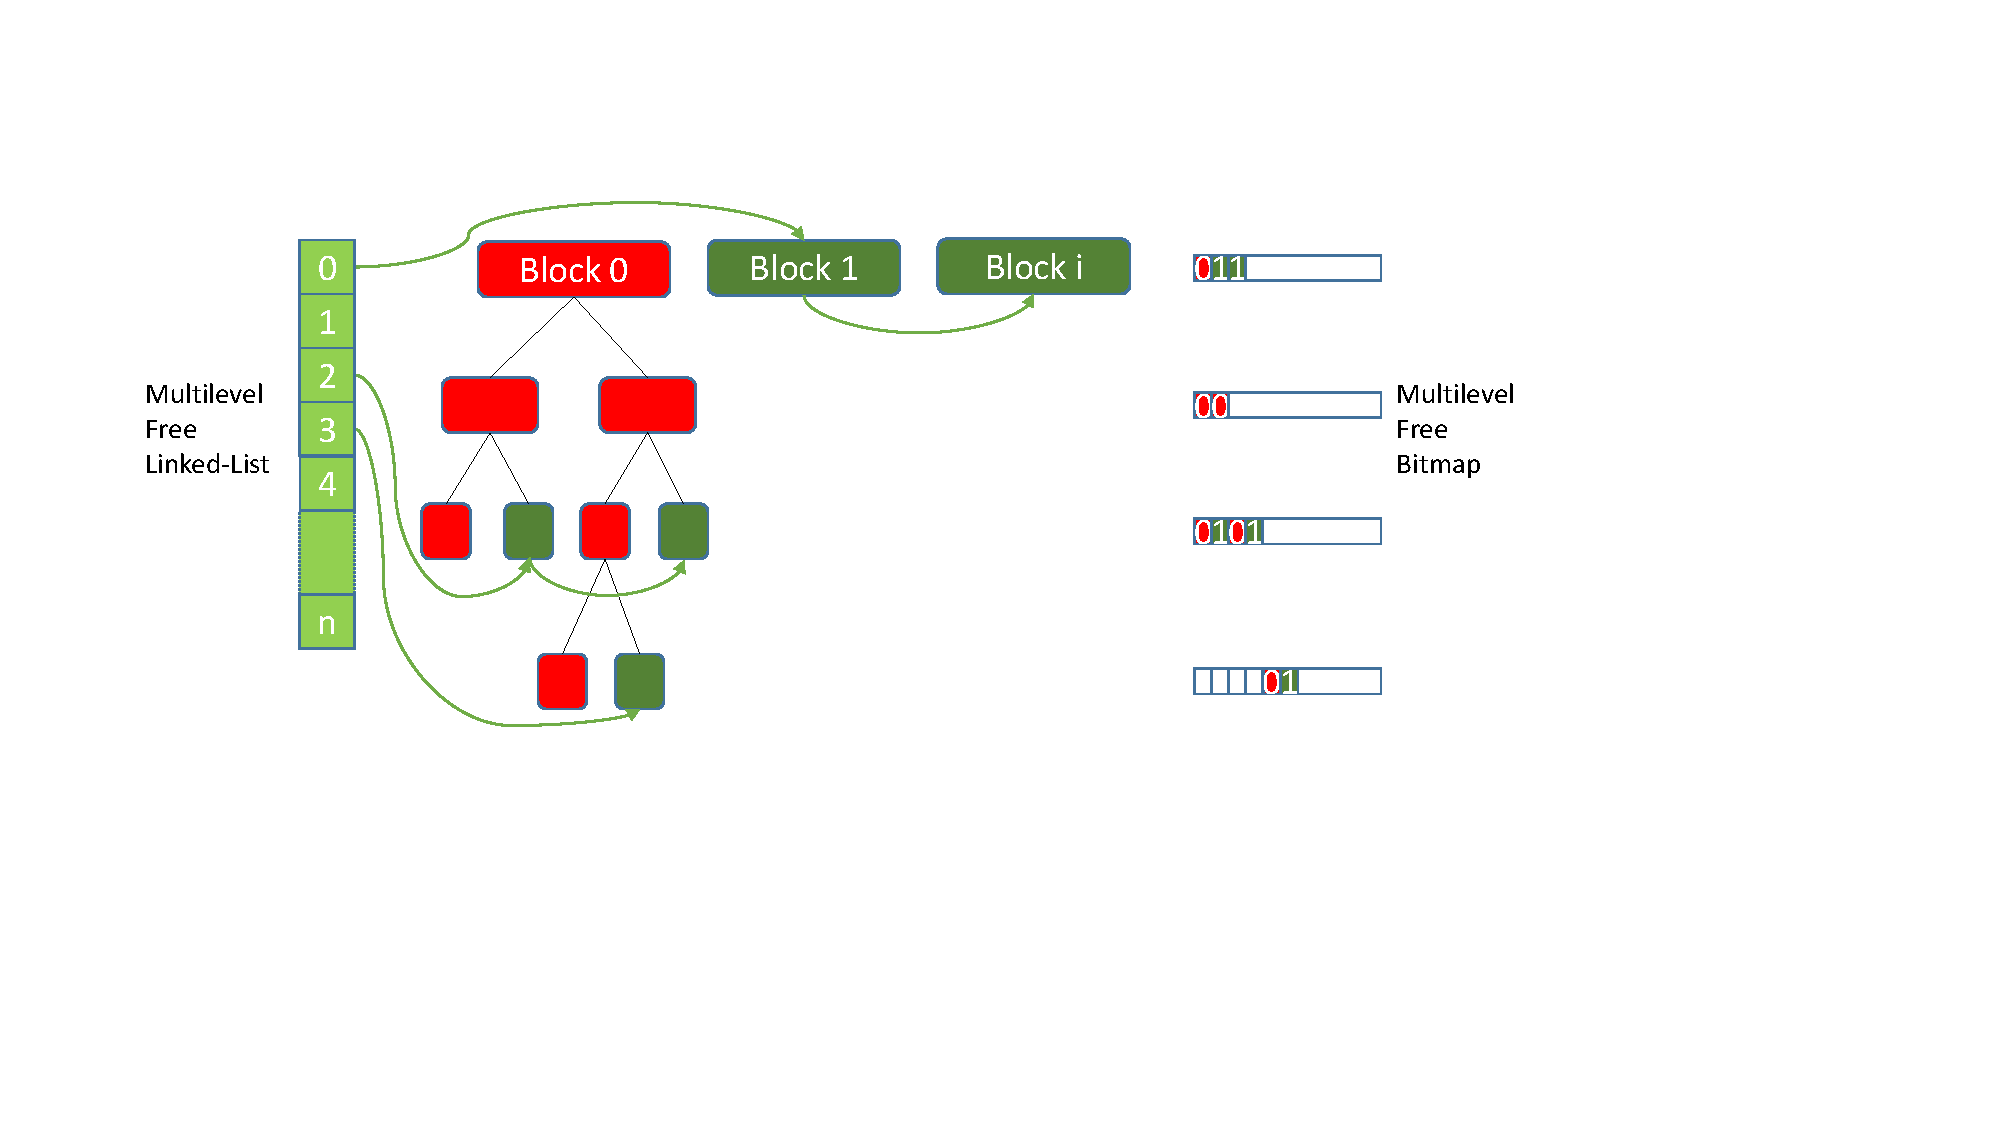
\includegraphics[width=0.7\textwidth]{fig3.pdf}
	\caption{Structures in Buddy Allocation Algorithms}
	\label{fig3}
\end{figure*}
In this section, we give the necessary backgrounds for buddy memory allocation algorithms and Isabelle/HOL theorem prover.

\subsection{Buddy Allocation Algorithms}\label{sec:buddy}
The buddy allocation algorithm~\cite{reg_knuth} aims to minimize external fragmentation by partitioning the memory into blocks fitting as best as possible memory requests from applications. Starting from an initial block with capacity equal to the maximum available memory $\Omega$, blocks are split into a power-of-two number of blocks $\Gamma$ to ease address computation. Each of the split blocks are buddies of each other and will be coalesce into a single block whenever is possible when disposing an allocated block. 

This mechanism logically organizes the memory into levels, where each level $l$ hosts $\Gamma^l$ blocks of equal size $\Omega/{\Gamma}^l$. Assuming the maximum memory $\Omega$ is a constant, it is easy to show that the level containing blocks with the necessary capacity to satisfy a memory request of size $s$ is $\Delta_s \equiv \lceil log_\Gamma (\Omega/  s) \rceil$ where $\lceil n \rceil$ is the upper natural number of $n$. 

For efficiency when accessing the free available blocks of a given allocation request, implementations use a multilevel linked-list to manage the free blocks on a given level. Under an allocation request of size $s$, if the linked list for the level $\Delta_s$ is not empty, a block is directly picked from the head of list. If it is (empty) the mechanism will try to find a higher level with free blocks and the splitting process starts to generate a perfect fit for the requested size. 

When a block is deallocated, the algorithms check whether the block can be merged with its buddy blocks. In this work, we provide a specification for the buddy allocator implemented in Zephyr, which uses quad-trees so $\Gamma = 4$.  Fig. \ref{fig3} describes a moment in memory system using multilevel free linked-list and multilevel free bitmap.



\subsection{Isabelle/HOL}
We use \correct{interactive theorem prover Isabelle/HOL}{the Isabelle/HOL interactive theorem prover}~\cite{reg_Isabelle/HOL} to conduct the specification and verification of the memory management. Isabelle/HOL is a higher order logic theorem prover, using a typed lambda calculus-like functional language for specifications.

Isabelle/HOL includes a specification for simple common types such as naturals (\emph{nat}), integers (\emph{int}) and booleans (\emph{bool}). It also specifies some composed data types like tuples, records, lists and sets that are parametrized with other types. Isabelle provides the interface \emph{datatype} for the creation of user defined types based on type constructors. 

Isabelle provides functions on predefined types to access their members or to provide additional operations over them. In the following we describe those functions and types that we use along this work. A tuple is denoted as (\emph{$t_1$} $\times$ \emph{$t_2$}), projection functions \emph{fst} and \emph{snd} respectively return elements $t_1$ and $t_2$. Lists are defined as a datatype with an empty construct denoted with \emph{NIL} or $[]$, and a concatenation construct denoted with $\#$, where $x\#xs$ adds $x$ to the front of $xs$. The $i$th component of a list $as$ is written as $as!i$. Isabelle/HOL provides functions for definite and indefinite descriptions. Definitive description is represented by $THE\ x.\ P\ x$ and returns the element uniquely described by the predicate $P$, else it returns and undefined value. Indefinite description is represented by $SOME\ x.\, P\ x$, selecting a random element from the predicate $P$ that must describe at least one element, else it returns an arbitrary value.

Isabelle/HOL allows \correct{user}{users} to create non-recursive specifications using the command \emph{definition}, and to create recursive specifications using commands \emph{primrec} and \emph{recursive}.
